\documentclass[a4paper]{article}

\usepackage{amsthm, amsmath, amsfonts, amssymb, hyperref}
\usepackage{enumerate}
\usepackage{latexsym}
\usepackage{amssymb}
\usepackage{amstext}
\usepackage{fancyhdr}
\usepackage{graphicx}
\usepackage[toc,page,title,titletoc,header]{appendix}
\usepackage{color}
\usepackage{titlesec}
\usepackage{lastpage}
\usepackage{algorithm}  
\usepackage{algorithmic}
\usepackage{caption}
\usepackage{listings}
\usepackage{subcaption}

\usepackage{multirow}
\usepackage[text={150mm,200mm},top=30mm,bottom=15mm]{geometry}
\newtoks\team
\newtoks\tihao
%%%=============================================================================================
\begin{document}
\setcounter{page}{0}
\pagestyle{empty}
\team{39925}
\tihao{A}
\begin{center}
\begin{tabular}{c@{\hspace{1mm}}c}
  \multicolumn{2}{l}{For office use only}\\
  T1 & {\underline {\makebox[8em][s]{}}}\\
  T2 & {\underline {\makebox[8em][s]{}}}\\
  T3 & {\underline {\makebox[8em][s]{}}}\\
  T4 & {\underline {\makebox[8em][s]{}}}\\
\end{tabular}\hfill
\begin{tabular}{c}
  Team Control Number\\
  \multirow{2}*{\textbf{\Huge \the\team}}\\
  \\
  Problem Chosen\\
  {\textbf{\huge \the\tihao }}\\
\end{tabular}\hfill
\begin{tabular}{c@{\hspace{1mm}}c}
  \multicolumn{2}{l}{For office use only}\\
  F1 & {\underline {\makebox[8em][s]{}}}\\
  F2 & {\underline {\makebox[8em][s]{}}}\\
  F3 & {\underline {\makebox[8em][s]{}}}\\
  F4 & {\underline {\makebox[8em][s]{}}}\\
\end{tabular}
\end{center}

\addvspace{1.5cm}

\begin{center}
\textbf{2015 Mathematical Contest in Modeling (MCM) Summary Sheet} \newline
(Attach a copy of this page to each copy of your solution paper.)
\end{center}

\begin{center}
Type a summary of your results on this page. Do not include \newline
the name of your school, advisor, or team members on this page. \newline

\end{center}

\begin{center}
\textbf{HICD Model: Eradication of Ebola in Ten Days}
\end{center}
\setlength{\parindent}{0pt} \setlength{\parskip}{1.5ex plus 0.5ex
minus 0.2ex}
In this paper, we start by presenting a complete \textbf{HICD Model} in explaining the interactive dynamical system of Ebola infection and the new medication breakthrough. The model characterizes the entire population into four categories: the Healthy(H), the Infected(I), the Cureless(C), and the Death(D). By solving the \textbf{discrete-time linear system of first-order difference equations}, we come up with the theoretical proposition that there exists at least one solution for the new medication to eliminate Ebola virus infection.

To minimize the total number of deaths in the Ebola elimination process, we then move on to develop a model employing a \textbf{marginal utility of medicine (MUM)} principle for the distribution priority of 61 affected districts in West Africa. We distribute the medicine based on how many lives an incremental unit of medicine can save from deteriorating into cureless in a given district. The medicines are divided up inclined to the district with the highest MUM. It is theoretically established that the lower bound of the total fatality number can be obtained by applying this MUM priority rule.

Depending on two possible locations of the medicine distributor, optimal delivery systems are proposed. If the World Medicine Association acts as the single overseas distributor, transportation can be reasonably curtailed by sending the medicine to adjacent districts. If there are multiple African laboratory distributors in Guinea, \textbf{simplex algorithm} is adopted for the optimization of the transportation costs by transforming the delivery system into a typical linear program. 

At the final stage, we implement a \textbf{computer simulation} to generate the EVD spreading pattern based on our HICD model, and test our two medicine distribution strategies against real Ebola data from WHO. The result is striking: keeping the recipient district’s level of preparedness constant, independent of the location of the medicine distributor, the EVD can be controlled within 10 days, the minimum death is stable at 520 people and the optimal daily production of medicine is around 6000 units per day. Our result also has public policy implication, namely, the level of preparedness of the recipient district should be above 50\% by WHO standard to make the implementation of the new medication genuinely effective.

\begin{figure}[htbp]
  	\centering
      	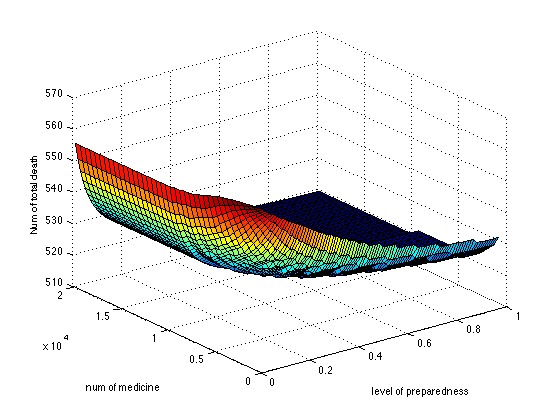
\includegraphics[width=0.4\textwidth]{figures/imgpMedDeath1.png}
      	\label{figure_3dDeath1}
      	\label{figure_3d}
\end{figure}


\end{document}
